\documentclass[1p]{elsarticle_modified}
%\bibliographystyle{elsarticle-num}

%\usepackage[colorlinks]{hyperref}
%\usepackage{abbrmath_seonhwa} %\Abb, \Ascr, \Acal ,\Abf, \Afrak
\usepackage{amsfonts}
\usepackage{amssymb}
\usepackage{amsmath}
\usepackage{amsthm}
\usepackage{scalefnt}
\usepackage{amsbsy}
\usepackage{kotex}
\usepackage{caption}
\usepackage{subfig}
\usepackage{color}
\usepackage{graphicx}
\usepackage{xcolor} %% white, black, red, green, blue, cyan, magenta, yellow
\usepackage{float}
\usepackage{setspace}
\usepackage{hyperref}

\usepackage{tikz}
\usetikzlibrary{arrows}

\usepackage{multirow}
\usepackage{array} % fixed length table
\usepackage{hhline}

%%%%%%%%%%%%%%%%%%%%%
\makeatletter
\renewcommand*\env@matrix[1][\arraystretch]{%
	\edef\arraystretch{#1}%
	\hskip -\arraycolsep
	\let\@ifnextchar\new@ifnextchar
	\array{*\c@MaxMatrixCols c}}
\makeatother %https://tex.stackexchange.com/questions/14071/how-can-i-increase-the-line-spacing-in-a-matrix
%%%%%%%%%%%%%%%

\usepackage[normalem]{ulem}

\newcommand{\msout}[1]{\ifmmode\text{\sout{\ensuremath{#1}}}\else\sout{#1}\fi}
%SOURCE: \msout is \stkout macro in https://tex.stackexchange.com/questions/20609/strikeout-in-math-mode

\newcommand{\cancel}[1]{
	\ifmmode
	{\color{red}\msout{#1}}
	\else
	{\color{red}\sout{#1}}
	\fi
}

\newcommand{\add}[1]{
	{\color{blue}\uwave{#1}}
}

\newcommand{\replace}[2]{
	\ifmmode
	{\color{red}\msout{#1}}{\color{blue}\uwave{#2}}
	\else
	{\color{red}\sout{#1}}{\color{blue}\uwave{#2}}
	\fi
}

\newcommand{\Sol}{\mathcal{S}} %segment
\newcommand{\D}{D} %diagram
\newcommand{\A}{\mathcal{A}} %arc


%%%%%%%%%%%%%%%%%%%%%%%%%%%%%5 test

\def\sl{\operatorname{\textup{SL}}(2,\Cbb)}
\def\psl{\operatorname{\textup{PSL}}(2,\Cbb)}
\def\quan{\mkern 1mu \triangleright \mkern 1mu}

\theoremstyle{definition}
\newtheorem{thm}{Theorem}[section]
\newtheorem{prop}[thm]{Proposition}
\newtheorem{lem}[thm]{Lemma}
\newtheorem{ques}[thm]{Question}
\newtheorem{cor}[thm]{Corollary}
\newtheorem{defn}[thm]{Definition}
\newtheorem{exam}[thm]{Example}
\newtheorem{rmk}[thm]{Remark}
\newtheorem{alg}[thm]{Algorithm}

\newcommand{\I}{\sqrt{-1}}
\begin{document}

%\begin{frontmatter}
%
%\title{Boundary parabolic representations of knots up to 8 crossings}
%
%%% Group authors per affiliation:
%\author{Yunhi Cho} 
%\address{Department of Mathematics, University of Seoul, Seoul, Korea}
%\ead{yhcho@uos.ac.kr}
%
%
%\author{Seonhwa Kim} %\fnref{s_kim}}
%\address{Center for Geometry and Physics, Institute for Basic Science, Pohang, 37673, Korea}
%\ead{ryeona17@ibs.re.kr}
%
%\author{Hyuk Kim}
%\address{Department of Mathematical Sciences, Seoul National University, Seoul 08826, Korea}
%\ead{hyukkim@snu.ac.kr}
%
%\author{Seokbeom Yoon}
%\address{Department of Mathematical Sciences, Seoul National University, Seoul, 08826,  Korea}
%\ead{sbyoon15@snu.ac.kr}
%
%\begin{abstract}
%We find all boundary parabolic representation of knots up to 8 crossings.
%
%\end{abstract}
%\begin{keyword}
%    \MSC[2010] 57M25 
%\end{keyword}
%
%\end{frontmatter}

%\linenumbers
%\tableofcontents
%
\newcommand\colored[1]{\textcolor{white}{\rule[-0.35ex]{0.8em}{1.4ex}}\kern-0.8em\color{red} #1}%
%\newcommand\colored[1]{\textcolor{white}{ #1}\kern-2.17ex	\textcolor{white}{ #1}\kern-1.81ex	\textcolor{white}{ #1}\kern-2.15ex\color{red}#1	}

{\Large $\underline{12n_{0090}~(K12n_{0090})}$}

\setlength{\tabcolsep}{10pt}
\renewcommand{\arraystretch}{1.6}
\vspace{1cm}\begin{tabular}{m{100pt}>{\centering\arraybackslash}m{274pt}}
\multirow{5}{120pt}{
	\centering
	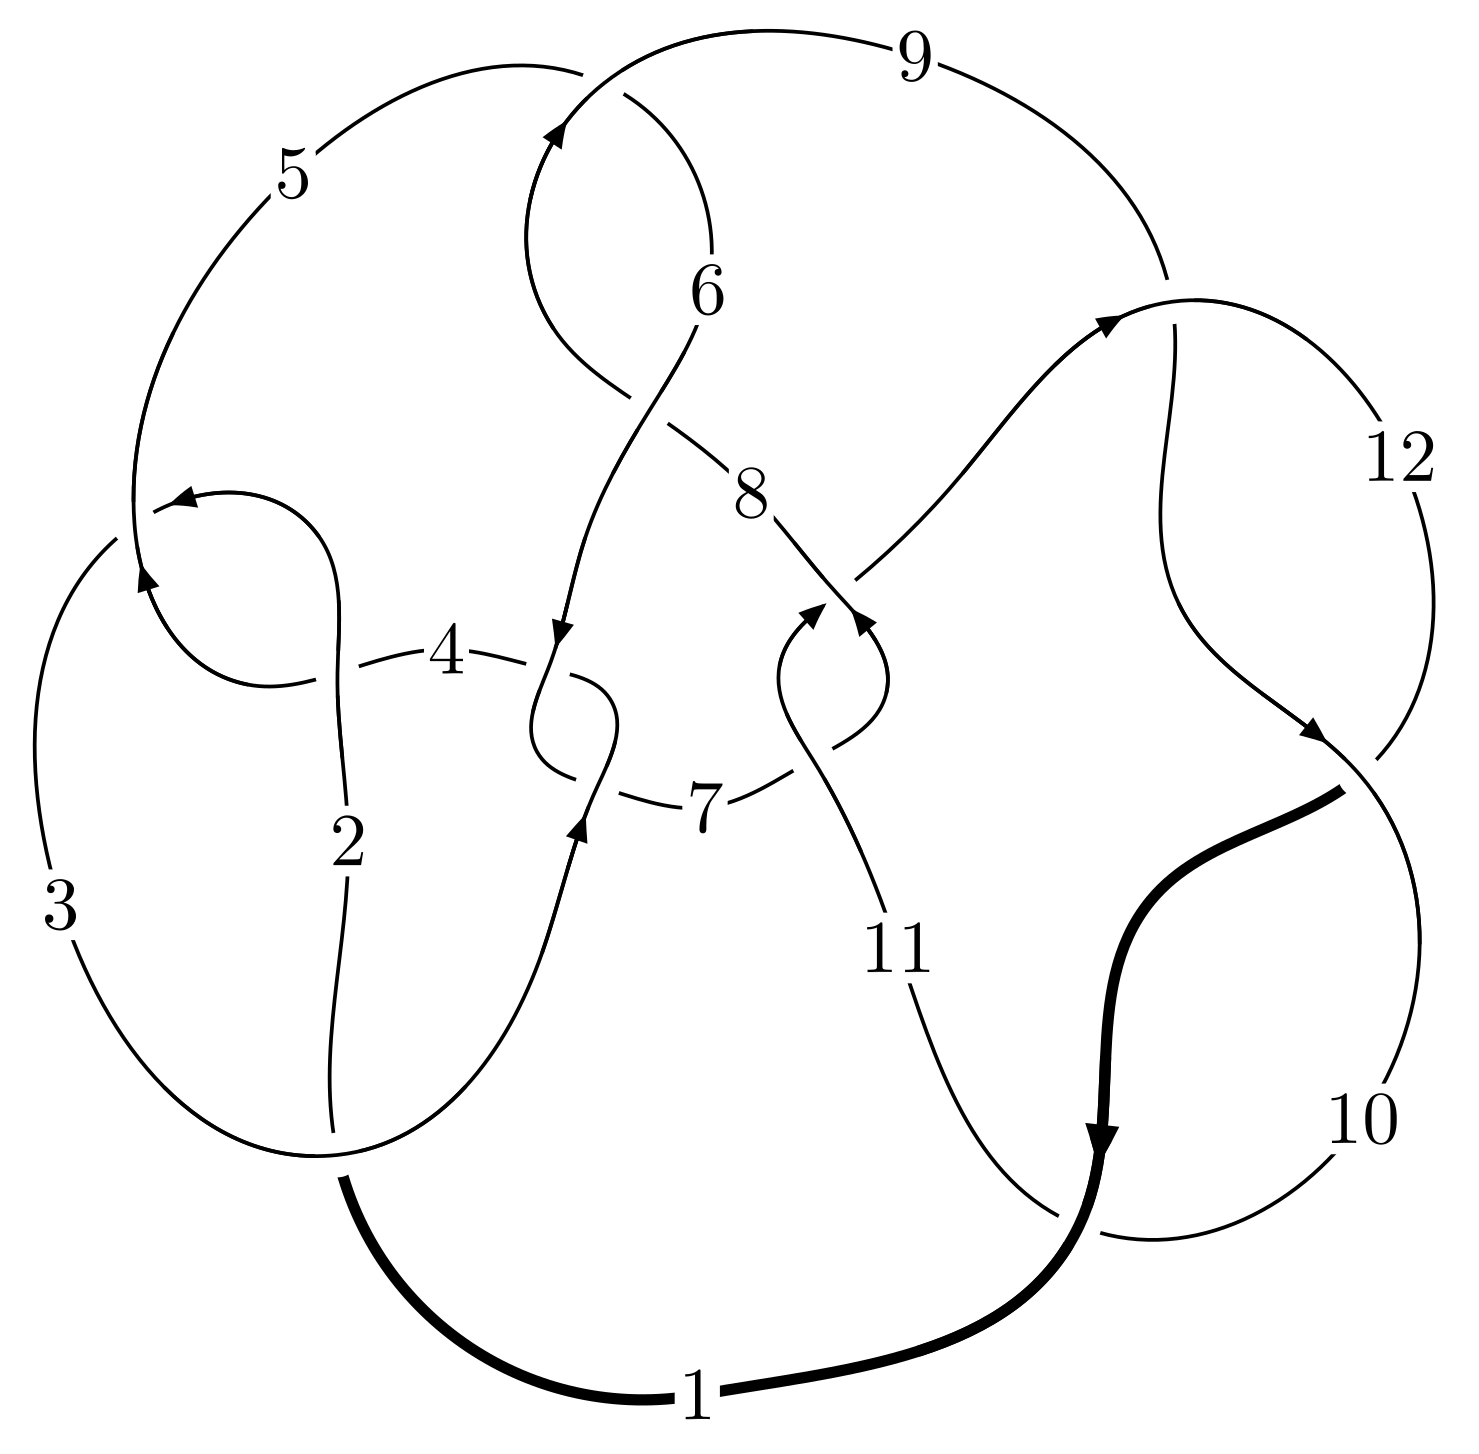
\includegraphics[width=112pt]{../../../GIT/diagram.site/Diagrams/png/2179_12n_0090.png}\\
\ \ \ A knot diagram\footnotemark}&
\allowdisplaybreaks
\textbf{Linearized knot diagam} \\
\cline{2-2}
 &
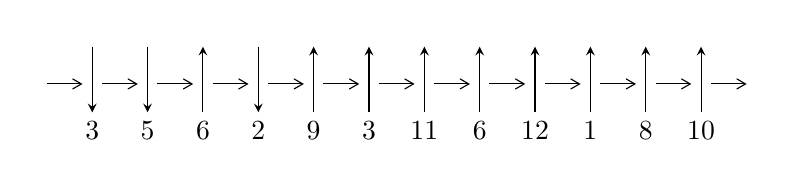
\begin{tikzpicture}[x=20pt, y=17pt]
	% nodes
	\node (C0) at (0, 0) {};
	\node (C1) at (1, 0) {};
	\node (C1U) at (1, +1) {};
	\node (C1D) at (1, -1) {3};

	\node (C2) at (2, 0) {};
	\node (C2U) at (2, +1) {};
	\node (C2D) at (2, -1) {5};

	\node (C3) at (3, 0) {};
	\node (C3U) at (3, +1) {};
	\node (C3D) at (3, -1) {6};

	\node (C4) at (4, 0) {};
	\node (C4U) at (4, +1) {};
	\node (C4D) at (4, -1) {2};

	\node (C5) at (5, 0) {};
	\node (C5U) at (5, +1) {};
	\node (C5D) at (5, -1) {9};

	\node (C6) at (6, 0) {};
	\node (C6U) at (6, +1) {};
	\node (C6D) at (6, -1) {3};

	\node (C7) at (7, 0) {};
	\node (C7U) at (7, +1) {};
	\node (C7D) at (7, -1) {11};

	\node (C8) at (8, 0) {};
	\node (C8U) at (8, +1) {};
	\node (C8D) at (8, -1) {6};

	\node (C9) at (9, 0) {};
	\node (C9U) at (9, +1) {};
	\node (C9D) at (9, -1) {12};

	\node (C10) at (10, 0) {};
	\node (C10U) at (10, +1) {};
	\node (C10D) at (10, -1) {1};

	\node (C11) at (11, 0) {};
	\node (C11U) at (11, +1) {};
	\node (C11D) at (11, -1) {8};

	\node (C12) at (12, 0) {};
	\node (C12U) at (12, +1) {};
	\node (C12D) at (12, -1) {10};
	\node (C13) at (13, 0) {};

	% arrows
	\draw[->,>={angle 60}]
	(C0) edge (C1) (C1) edge (C2) (C2) edge (C3) (C3) edge (C4) (C4) edge (C5) (C5) edge (C6) (C6) edge (C7) (C7) edge (C8) (C8) edge (C9) (C9) edge (C10) (C10) edge (C11) (C11) edge (C12) (C12) edge (C13) ;	\draw[->,>=stealth]
	(C1U) edge (C1D) (C2U) edge (C2D) (C3D) edge (C3U) (C4U) edge (C4D) (C5D) edge (C5U) (C6D) edge (C6U) (C7D) edge (C7U) (C8D) edge (C8U) (C9D) edge (C9U) (C10D) edge (C10U) (C11D) edge (C11U) (C12D) edge (C12U) ;
	\end{tikzpicture} \\
\hhline{~~} \\& 
\textbf{Solving Sequence} \\ \cline{2-2} 
 &
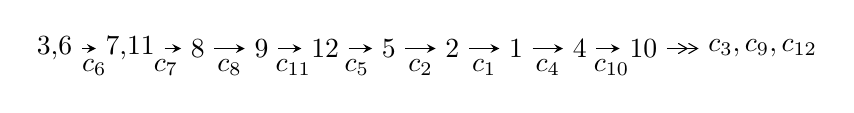
\begin{tikzpicture}[x=23pt, y=7pt]
	% node
	\node (A0) at (-1/8, 0) {3,6};
	\node (A1) at (17/16, 0) {7,11};
	\node (A2) at (17/8, 0) {8};
	\node (A3) at (25/8, 0) {9};
	\node (A4) at (33/8, 0) {12};
	\node (A5) at (41/8, 0) {5};
	\node (A6) at (49/8, 0) {2};
	\node (A7) at (57/8, 0) {1};
	\node (A8) at (65/8, 0) {4};
	\node (A9) at (73/8, 0) {10};
	\node (C1) at (1/2, -1) {$c_{6}$};
	\node (C2) at (13/8, -1) {$c_{7}$};
	\node (C3) at (21/8, -1) {$c_{8}$};
	\node (C4) at (29/8, -1) {$c_{11}$};
	\node (C5) at (37/8, -1) {$c_{5}$};
	\node (C6) at (45/8, -1) {$c_{2}$};
	\node (C7) at (53/8, -1) {$c_{1}$};
	\node (C8) at (61/8, -1) {$c_{4}$};
	\node (C9) at (69/8, -1) {$c_{10}$};
	\node (A10) at (11, 0) {$c_{3},c_{9},c_{12}$};

	% edge
	\draw[->,>=stealth]	
	(A0) edge (A1) (A1) edge (A2) (A2) edge (A3) (A3) edge (A4) (A4) edge (A5) (A5) edge (A6) (A6) edge (A7) (A7) edge (A8) (A8) edge (A9) ;
	\draw[->>,>={angle 60}]	
	(A9) edge (A10);
\end{tikzpicture} \\ 

\end{tabular} \\

\footnotetext{
The image of knot diagram is generated by the software ``\textbf{Draw programme}" developed by Andrew Bartholomew(\url{http://www.layer8.co.uk/maths/draw/index.htm\#Running-draw}), where we modified some parts for our purpose(\url{https://github.com/CATsTAILs/LinksPainter}).
}\phantom \\ \newline 
\centering \textbf{Ideals for irreducible components\footnotemark of $X_{\text{par}}$} 
 
\begin{align*}
I^u_{1}&=\langle 
9.96682\times10^{157} u^{51}+6.43522\times10^{157} u^{50}+\cdots+4.80775\times10^{159} b-2.81921\times10^{161},\\
\phantom{I^u_{1}}&\phantom{= \langle  }-8.50264\times10^{159} u^{51}-4.59905\times10^{160} u^{50}+\cdots+4.80775\times10^{159} a-2.25629\times10^{162},\\
\phantom{I^u_{1}}&\phantom{= \langle  }u^{52}+6 u^{51}+\cdots-384 u+256\rangle \\
I^u_{2}&=\langle 
- u^5+2 u^3+u^2+b-2 u-1,\;- u^5-2 u^4+u^3+3 u^2+a-2,\;u^6+u^5- u^4-2 u^3+u+1\rangle \\
\\
I^v_{1}&=\langle 
a,\;-435 v^7+1730 v^6+9811 v^5+13983 v^4+4411 v^3-5372 v^2+287 b-4318 v-1024,\\
\phantom{I^v_{1}}&\phantom{= \langle  }v^8-4 v^7-22 v^6-34 v^5-17 v^4+6 v^3+11 v^2+5 v+1\rangle \\
\end{align*}
\raggedright * 3 irreducible components of $\dim_{\mathbb{C}}=0$, with total 66 representations.\\
\footnotetext{All coefficients of polynomials are rational numbers. But the coefficients are sometimes approximated in decimal forms when there is not enough margin.}
\newpage
\renewcommand{\arraystretch}{1}
\centering \section*{I. $I^u_{1}= \langle 9.97\times10^{157} u^{51}+6.44\times10^{157} u^{50}+\cdots+4.81\times10^{159} b-2.82\times10^{161},\;-8.50\times10^{159} u^{51}-4.60\times10^{160} u^{50}+\cdots+4.81\times10^{159} a-2.26\times10^{162},\;u^{52}+6 u^{51}+\cdots-384 u+256 \rangle$}
\flushleft \textbf{(i) Arc colorings}\\
\begin{tabular}{m{7pt} m{180pt} m{7pt} m{180pt} }
\flushright $a_{3}=$&$\begin{pmatrix}0\\u\end{pmatrix}$ \\
\flushright $a_{6}=$&$\begin{pmatrix}1\\0\end{pmatrix}$ \\
\flushright $a_{7}=$&$\begin{pmatrix}1\\- u^2\end{pmatrix}$ \\
\flushright $a_{11}=$&$\begin{pmatrix}1.76853 u^{51}+9.56590 u^{50}+\cdots-2926.51 u+469.302\\-0.0207307 u^{51}-0.0133851 u^{50}+\cdots-241.958 u+58.6388\end{pmatrix}$ \\
\flushright $a_{8}=$&$\begin{pmatrix}1.11147 u^{51}+6.04469 u^{50}+\cdots-1943.07 u+322.353\\1.41662 u^{51}+7.57791 u^{50}+\cdots-1710.65 u+565.183\end{pmatrix}$ \\
\flushright $a_{9}=$&$\begin{pmatrix}2.52808 u^{51}+13.6226 u^{50}+\cdots-3653.72 u+887.535\\1.41662 u^{51}+7.57791 u^{50}+\cdots-1710.65 u+565.183\end{pmatrix}$ \\
\flushright $a_{12}=$&$\begin{pmatrix}2.24827 u^{51}+12.0747 u^{50}+\cdots-3114.80 u+728.310\\2.81685 u^{51}+15.1244 u^{50}+\cdots-3490.75 u+1142.79\end{pmatrix}$ \\
\flushright $a_{5}=$&$\begin{pmatrix}-0.522374 u^{51}-2.76840 u^{50}+\cdots+479.530 u-230.084\\-1.17566 u^{51}-6.25747 u^{50}+\cdots+1309.09 u-442.421\end{pmatrix}$ \\
\flushright $a_{2}=$&$\begin{pmatrix}-0.653284 u^{51}-3.48907 u^{50}+\cdots+829.556 u-212.337\\-1.17566 u^{51}-6.25747 u^{50}+\cdots+1309.09 u-442.421\end{pmatrix}$ \\
\flushright $a_{1}=$&$\begin{pmatrix}-0.653284 u^{51}-3.48907 u^{50}+\cdots+829.556 u-212.337\\-0.883950 u^{51}-4.70152 u^{50}+\cdots+976.480 u-332.178\end{pmatrix}$ \\
\flushright $a_{4}=$&$\begin{pmatrix}u\\u\end{pmatrix}$ \\
\flushright $a_{10}=$&$\begin{pmatrix}2.40012 u^{51}+12.9314 u^{50}+\cdots-3603.52 u+730.563\\1.81072 u^{51}+9.76249 u^{50}+\cdots-2349.30 u+761.984\end{pmatrix}$\\&\end{tabular}
\flushleft \textbf{(ii) Obstruction class $= -1$}\\~\\
\flushleft \textbf{(iii) Cusp Shapes $= 3.23763 u^{51}+16.6512 u^{50}+\cdots-115.091 u+1897.90$}\\~\\
\newpage\renewcommand{\arraystretch}{1}
\flushleft \textbf{(iv) u-Polynomials at the component}\newline \\
\begin{tabular}{m{50pt}|m{274pt}}
Crossings & \hspace{64pt}u-Polynomials at each crossing \\
\hline $$\begin{aligned}c_{1}\end{aligned}$$&$\begin{aligned}
&u^{52}+14 u^{51}+\cdots+1402 u+1
\end{aligned}$\\
\hline $$\begin{aligned}c_{2},c_{4}\end{aligned}$$&$\begin{aligned}
&u^{52}-10 u^{51}+\cdots-42 u+1
\end{aligned}$\\
\hline $$\begin{aligned}c_{3},c_{6}\end{aligned}$$&$\begin{aligned}
&u^{52}+6 u^{51}+\cdots-384 u+256
\end{aligned}$\\
\hline $$\begin{aligned}c_{5},c_{8}\end{aligned}$$&$\begin{aligned}
&u^{52}+3 u^{51}+\cdots+2 u+1
\end{aligned}$\\
\hline $$\begin{aligned}c_{7},c_{11}\end{aligned}$$&$\begin{aligned}
&u^{52}-2 u^{51}+\cdots-192 u+64
\end{aligned}$\\
\hline $$\begin{aligned}c_{9},c_{10},c_{12}\end{aligned}$$&$\begin{aligned}
&u^{52}+8 u^{51}+\cdots+5 u+1
\end{aligned}$\\
\hline
\end{tabular}\\~\\
\newpage\renewcommand{\arraystretch}{1}
\flushleft \textbf{(v) Riley Polynomials at the component}\newline \\
\begin{tabular}{m{50pt}|m{274pt}}
Crossings & \hspace{64pt}Riley Polynomials at each crossing \\
\hline $$\begin{aligned}c_{1}\end{aligned}$$&$\begin{aligned}
&y^{52}+58 y^{51}+\cdots-1883250 y+1
\end{aligned}$\\
\hline $$\begin{aligned}c_{2},c_{4}\end{aligned}$$&$\begin{aligned}
&y^{52}-14 y^{51}+\cdots-1402 y+1
\end{aligned}$\\
\hline $$\begin{aligned}c_{3},c_{6}\end{aligned}$$&$\begin{aligned}
&y^{52}-54 y^{51}+\cdots-6144000 y+65536
\end{aligned}$\\
\hline $$\begin{aligned}c_{5},c_{8}\end{aligned}$$&$\begin{aligned}
&y^{52}+11 y^{51}+\cdots-2 y+1
\end{aligned}$\\
\hline $$\begin{aligned}c_{7},c_{11}\end{aligned}$$&$\begin{aligned}
&y^{52}-42 y^{51}+\cdots+4096 y+4096
\end{aligned}$\\
\hline $$\begin{aligned}c_{9},c_{10},c_{12}\end{aligned}$$&$\begin{aligned}
&y^{52}-56 y^{51}+\cdots-11 y+1
\end{aligned}$\\
\hline
\end{tabular}\\~\\
\newpage\flushleft \textbf{(vi) Complex Volumes and Cusp Shapes}
$$\begin{array}{c|c|c}  
\text{Solutions to }I^u_{1}& \I (\text{vol} + \sqrt{-1}CS) & \text{Cusp shape}\\
 \hline 
\begin{aligned}
u &= -0.894300 + 0.467621 I \\
a &= \phantom{-}1.21589 + 0.98600 I \\
b &= -0.940205 + 0.671189 I\end{aligned}
 & -2.35126 + 1.18530 I & \phantom{-0.000000 } 0 \\ \hline\begin{aligned}
u &= -0.894300 - 0.467621 I \\
a &= \phantom{-}1.21589 - 0.98600 I \\
b &= -0.940205 - 0.671189 I\end{aligned}
 & -2.35126 - 1.18530 I & \phantom{-0.000000 } 0 \\ \hline\begin{aligned}
u &= -0.077034 + 0.976513 I \\
a &= -0.541763 + 0.843119 I \\
b &= \phantom{-}0.924664 + 0.513211 I\end{aligned}
 & \phantom{-}8.16733 - 1.74753 I & \phantom{-0.000000 } 0 \\ \hline\begin{aligned}
u &= -0.077034 - 0.976513 I \\
a &= -0.541763 - 0.843119 I \\
b &= \phantom{-}0.924664 - 0.513211 I\end{aligned}
 & \phantom{-}8.16733 + 1.74753 I & \phantom{-0.000000 } 0 \\ \hline\begin{aligned}
u &= \phantom{-}0.311772 + 0.824230 I \\
a &= -0.61198 - 1.93647 I \\
b &= -1.362440 - 0.024471 I\end{aligned}
 & \phantom{-}2.07038 + 1.52953 I & \phantom{-}6.00000 - 4.40429 I \\ \hline\begin{aligned}
u &= \phantom{-}0.311772 - 0.824230 I \\
a &= -0.61198 + 1.93647 I \\
b &= -1.362440 + 0.024471 I\end{aligned}
 & \phantom{-}2.07038 - 1.52953 I & \phantom{-}6.00000 + 4.40429 I \\ \hline\begin{aligned}
u &= -0.349211 + 0.778404 I \\
a &= \phantom{-}0.893037 + 0.518298 I \\
b &= \phantom{-}0.299421 + 0.403800 I\end{aligned}
 & -1.82480 + 1.05655 I & -2.50386 - 1.55405 I \\ \hline\begin{aligned}
u &= -0.349211 - 0.778404 I \\
a &= \phantom{-}0.893037 - 0.518298 I \\
b &= \phantom{-}0.299421 - 0.403800 I\end{aligned}
 & -1.82480 - 1.05655 I & -2.50386 + 1.55405 I \\ \hline\begin{aligned}
u &= \phantom{-}0.212493 + 1.195980 I \\
a &= \phantom{-}0.789348 + 0.054066 I \\
b &= \phantom{-}2.03489 - 0.17085 I\end{aligned}
 & \phantom{-}0.23912 + 3.31860 I & \phantom{-0.000000 } 0 \\ \hline\begin{aligned}
u &= \phantom{-}0.212493 - 1.195980 I \\
a &= \phantom{-}0.789348 - 0.054066 I \\
b &= \phantom{-}2.03489 + 0.17085 I\end{aligned}
 & \phantom{-}0.23912 - 3.31860 I & \phantom{-0.000000 } 0\\
 \hline 
 \end{array}$$\newpage$$\begin{array}{c|c|c}  
\text{Solutions to }I^u_{1}& \I (\text{vol} + \sqrt{-1}CS) & \text{Cusp shape}\\
 \hline 
\begin{aligned}
u &= \phantom{-}1.197920 + 0.212460 I \\
a &= \phantom{-}0.1235270 + 0.0251718 I \\
b &= -0.208678 - 0.717859 I\end{aligned}
 & \phantom{-}2.51889 + 0.64898 I & \phantom{-0.000000 } 0 \\ \hline\begin{aligned}
u &= \phantom{-}1.197920 - 0.212460 I \\
a &= \phantom{-}0.1235270 - 0.0251718 I \\
b &= -0.208678 + 0.717859 I\end{aligned}
 & \phantom{-}2.51889 - 0.64898 I & \phantom{-0.000000 } 0 \\ \hline\begin{aligned}
u &= \phantom{-}0.742980\phantom{ +0.000000I} \\
a &= \phantom{-}4.08088\phantom{ +0.000000I} \\
b &= -0.756924\phantom{ +0.000000I}\end{aligned}
 & \phantom{-}6.40671\phantom{ +0.000000I} & \phantom{-}22.8380\phantom{ +0.000000I} \\ \hline\begin{aligned}
u &= -0.678225 + 0.259653 I \\
a &= -0.219400 - 0.219932 I \\
b &= -0.735304 + 0.665653 I\end{aligned}
 & \phantom{-}0.98837 - 7.05447 I & \phantom{-}10.8678 + 11.9178 I \\ \hline\begin{aligned}
u &= -0.678225 - 0.259653 I \\
a &= -0.219400 + 0.219932 I \\
b &= -0.735304 - 0.665653 I\end{aligned}
 & \phantom{-}0.98837 + 7.05447 I & \phantom{-}10.8678 - 11.9178 I \\ \hline\begin{aligned}
u &= -1.185680 + 0.489419 I \\
a &= -0.0714715 + 0.0415507 I \\
b &= \phantom{-}0.018026 + 0.520754 I\end{aligned}
 & \phantom{-}1.02907 - 5.96168 I & \phantom{-0.000000 } 0 \\ \hline\begin{aligned}
u &= -1.185680 - 0.489419 I \\
a &= -0.0714715 - 0.0415507 I \\
b &= \phantom{-}0.018026 - 0.520754 I\end{aligned}
 & \phantom{-}1.02907 + 5.96168 I & \phantom{-0.000000 } 0 \\ \hline\begin{aligned}
u &= -0.661772 + 0.025420 I \\
a &= \phantom{-}0.573044 + 0.203692 I \\
b &= \phantom{-}0.601130 - 0.866198 I\end{aligned}
 & -3.01505 - 2.93991 I & \phantom{-}8.02854 + 4.94099 I \\ \hline\begin{aligned}
u &= -0.661772 - 0.025420 I \\
a &= \phantom{-}0.573044 - 0.203692 I \\
b &= \phantom{-}0.601130 + 0.866198 I\end{aligned}
 & -3.01505 + 2.93991 I & \phantom{-}8.02854 - 4.94099 I \\ \hline\begin{aligned}
u &= -0.608562 + 0.052862 I \\
a &= -1.204570 - 0.413046 I \\
b &= -0.295631 + 0.903933 I\end{aligned}
 & \phantom{-}0.61020 + 1.37415 I & \phantom{-}10.26914 - 1.41740 I\\
 \hline 
 \end{array}$$\newpage$$\begin{array}{c|c|c}  
\text{Solutions to }I^u_{1}& \I (\text{vol} + \sqrt{-1}CS) & \text{Cusp shape}\\
 \hline 
\begin{aligned}
u &= -0.608562 - 0.052862 I \\
a &= -1.204570 + 0.413046 I \\
b &= -0.295631 - 0.903933 I\end{aligned}
 & \phantom{-}0.61020 - 1.37415 I & \phantom{-}10.26914 + 1.41740 I \\ \hline\begin{aligned}
u &= \phantom{-}0.603802\phantom{ +0.000000I} \\
a &= -0.298164\phantom{ +0.000000I} \\
b &= \phantom{-}1.06305\phantom{ +0.000000I}\end{aligned}
 & \phantom{-}5.57235\phantom{ +0.000000I} & \phantom{-}20.0660\phantom{ +0.000000I} \\ \hline\begin{aligned}
u &= \phantom{-}0.032656 + 0.593010 I \\
a &= -0.36952 - 1.62271 I \\
b &= -0.996072 - 0.539949 I\end{aligned}
 & \phantom{-}0.524938 - 0.113527 I & \phantom{-}8.64384 + 0.42173 I \\ \hline\begin{aligned}
u &= \phantom{-}0.032656 - 0.593010 I \\
a &= -0.36952 + 1.62271 I \\
b &= -0.996072 + 0.539949 I\end{aligned}
 & \phantom{-}0.524938 + 0.113527 I & \phantom{-}8.64384 - 0.42173 I \\ \hline\begin{aligned}
u &= -0.403944 + 0.310632 I \\
a &= -7.08832 - 3.53754 I \\
b &= \phantom{-}1.05119 - 1.20630 I\end{aligned}
 & -0.279878 + 0.575640 I & \phantom{-}9.6300 + 22.9731 I \\ \hline\begin{aligned}
u &= -0.403944 - 0.310632 I \\
a &= -7.08832 + 3.53754 I \\
b &= \phantom{-}1.05119 + 1.20630 I\end{aligned}
 & -0.279878 - 0.575640 I & \phantom{-}9.6300 - 22.9731 I \\ \hline\begin{aligned}
u &= \phantom{-}1.63347 + 0.20317 I \\
a &= -1.33849 + 0.48910 I \\
b &= \phantom{-}2.46513 - 0.73973 I\end{aligned}
 & \phantom{-}6.81089 + 3.11557 I & \phantom{-0.000000 } 0 \\ \hline\begin{aligned}
u &= \phantom{-}1.63347 - 0.20317 I \\
a &= -1.33849 - 0.48910 I \\
b &= \phantom{-}2.46513 + 0.73973 I\end{aligned}
 & \phantom{-}6.81089 - 3.11557 I & \phantom{-0.000000 } 0 \\ \hline\begin{aligned}
u &= -1.61892 + 0.31042 I \\
a &= -1.45018 - 0.02409 I \\
b &= \phantom{-}2.18977 - 1.46329 I\end{aligned}
 & \phantom{-}6.62010 - 3.75962 I & \phantom{-0.000000 } 0 \\ \hline\begin{aligned}
u &= -1.61892 - 0.31042 I \\
a &= -1.45018 + 0.02409 I \\
b &= \phantom{-}2.18977 + 1.46329 I\end{aligned}
 & \phantom{-}6.62010 + 3.75962 I & \phantom{-0.000000 } 0\\
 \hline 
 \end{array}$$\newpage$$\begin{array}{c|c|c}  
\text{Solutions to }I^u_{1}& \I (\text{vol} + \sqrt{-1}CS) & \text{Cusp shape}\\
 \hline 
\begin{aligned}
u &= \phantom{-}1.60931 + 0.54791 I \\
a &= \phantom{-}1.042880 - 0.658926 I \\
b &= -2.04032 + 0.38768 I\end{aligned}
 & \phantom{-}13.6500 + 7.8231 I & \phantom{-0.000000 } 0 \\ \hline\begin{aligned}
u &= \phantom{-}1.60931 - 0.54791 I \\
a &= \phantom{-}1.042880 + 0.658926 I \\
b &= -2.04032 - 0.38768 I\end{aligned}
 & \phantom{-}13.6500 - 7.8231 I & \phantom{-0.000000 } 0 \\ \hline\begin{aligned}
u &= -1.70298 + 0.07577 I \\
a &= \phantom{-}1.201980 + 0.256516 I \\
b &= -1.81377 - 1.00382 I\end{aligned}
 & \phantom{-}14.7382 - 0.7846 I & \phantom{-0.000000 } 0 \\ \hline\begin{aligned}
u &= -1.70298 - 0.07577 I \\
a &= \phantom{-}1.201980 - 0.256516 I \\
b &= -1.81377 + 1.00382 I\end{aligned}
 & \phantom{-}14.7382 + 0.7846 I & \phantom{-0.000000 } 0 \\ \hline\begin{aligned}
u &= -1.67977 + 0.44939 I \\
a &= \phantom{-}0.0708644 - 0.1108210 I \\
b &= -0.179650 - 1.147460 I\end{aligned}
 & \phantom{-}8.63174 - 7.01563 I & \phantom{-0.000000 } 0 \\ \hline\begin{aligned}
u &= -1.67977 - 0.44939 I \\
a &= \phantom{-}0.0708644 + 0.1108210 I \\
b &= -0.179650 + 1.147460 I\end{aligned}
 & \phantom{-}8.63174 + 7.01563 I & \phantom{-0.000000 } 0 \\ \hline\begin{aligned}
u &= -1.64583 + 0.58571 I \\
a &= \phantom{-}1.39373 + 0.38788 I \\
b &= -2.58601 + 1.40311 I\end{aligned}
 & \phantom{-}6.05959 - 10.09710 I & \phantom{-0.000000 } 0 \\ \hline\begin{aligned}
u &= -1.64583 - 0.58571 I \\
a &= \phantom{-}1.39373 - 0.38788 I \\
b &= -2.58601 - 1.40311 I\end{aligned}
 & \phantom{-}6.05959 + 10.09710 I & \phantom{-0.000000 } 0 \\ \hline\begin{aligned}
u &= \phantom{-}1.75625 + 0.06042 I \\
a &= -0.147310 + 0.027996 I \\
b &= \phantom{-}0.59079 - 1.50355 I\end{aligned}
 & \phantom{-}9.30042 + 0.19617 I & \phantom{-0.000000 } 0 \\ \hline\begin{aligned}
u &= \phantom{-}1.75625 - 0.06042 I \\
a &= -0.147310 - 0.027996 I \\
b &= \phantom{-}0.59079 + 1.50355 I\end{aligned}
 & \phantom{-}9.30042 - 0.19617 I & \phantom{-0.000000 } 0\\
 \hline 
 \end{array}$$\newpage$$\begin{array}{c|c|c}  
\text{Solutions to }I^u_{1}& \I (\text{vol} + \sqrt{-1}CS) & \text{Cusp shape}\\
 \hline 
\begin{aligned}
u &= \phantom{-}1.77632 + 0.13695 I \\
a &= \phantom{-}1.402470 + 0.047674 I \\
b &= -2.98413 - 0.73221 I\end{aligned}
 & \phantom{-}7.28875 + 2.86108 I & \phantom{-0.000000 } 0 \\ \hline\begin{aligned}
u &= \phantom{-}1.77632 - 0.13695 I \\
a &= \phantom{-}1.402470 - 0.047674 I \\
b &= -2.98413 + 0.73221 I\end{aligned}
 & \phantom{-}7.28875 - 2.86108 I & \phantom{-0.000000 } 0 \\ \hline\begin{aligned}
u &= \phantom{-}0.164240\phantom{ +0.000000I} \\
a &= \phantom{-}2.46011\phantom{ +0.000000I} \\
b &= -0.653644\phantom{ +0.000000I}\end{aligned}
 & \phantom{-}0.823260\phantom{ +0.000000I} & \phantom{-}12.0980\phantom{ +0.000000I} \\ \hline\begin{aligned}
u &= \phantom{-}0.155157\phantom{ +0.000000I} \\
a &= -45.9491\phantom{ +0.000000I} \\
b &= \phantom{-}0.488931\phantom{ +0.000000I}\end{aligned}
 & -0.760272\phantom{ +0.000000I} & \phantom{-}181.970\phantom{ +0.000000I} \\ \hline\begin{aligned}
u &= -1.72375 + 0.82810 I \\
a &= -1.145390 - 0.563607 I \\
b &= \phantom{-}2.67815 - 1.22216 I\end{aligned}
 & \phantom{-}13.0011 - 15.0944 I & \phantom{-0.000000 } 0 \\ \hline\begin{aligned}
u &= -1.72375 - 0.82810 I \\
a &= -1.145390 + 0.563607 I \\
b &= \phantom{-}2.67815 + 1.22216 I\end{aligned}
 & \phantom{-}13.0011 + 15.0944 I & \phantom{-0.000000 } 0 \\ \hline\begin{aligned}
u &= -1.62576 + 1.11014 I \\
a &= -0.700530 - 0.381882 I \\
b &= \phantom{-}0.99337 - 2.09354 I\end{aligned}
 & \phantom{-}3.67025 + 2.14792 I & \phantom{-0.000000 } 0 \\ \hline\begin{aligned}
u &= -1.62576 - 1.11014 I \\
a &= -0.700530 + 0.381882 I \\
b &= \phantom{-}0.99337 + 2.09354 I\end{aligned}
 & \phantom{-}3.67025 - 2.14792 I & \phantom{-0.000000 } 0 \\ \hline\begin{aligned}
u &= \phantom{-}0.38941 + 1.93312 I \\
a &= -0.392879 + 0.204474 I \\
b &= -2.57270 + 1.01210 I\end{aligned}
 & \phantom{-}7.15465 + 5.75608 I & \phantom{-0.000000 } 0 \\ \hline\begin{aligned}
u &= \phantom{-}0.38941 - 1.93312 I \\
a &= -0.392879 - 0.204474 I \\
b &= -2.57270 - 1.01210 I\end{aligned}
 & \phantom{-}7.15465 - 5.75608 I & \phantom{-0.000000 } 0\\
 \hline 
 \end{array}$$\newpage$$\begin{array}{c|c|c}  
\text{Solutions to }I^u_{1}& \I (\text{vol} + \sqrt{-1}CS) & \text{Cusp shape}\\
 \hline 
\begin{aligned}
u &= \phantom{-}2.10305 + 0.45567 I \\
a &= -1.071810 + 0.220002 I \\
b &= \phantom{-}3.29768 + 0.55847 I\end{aligned}
 & \phantom{-}15.0358 + 7.1240 I & \phantom{-0.000000 } 0 \\ \hline\begin{aligned}
u &= \phantom{-}2.10305 - 0.45567 I \\
a &= -1.071810 - 0.220002 I \\
b &= \phantom{-}3.29768 - 0.55847 I\end{aligned}
 & \phantom{-}15.0358 - 7.1240 I & \phantom{-0.000000 } 0\\
 \hline 
 \end{array}$$\newpage\newpage\renewcommand{\arraystretch}{1}
\centering \section*{II. $I^u_{2}= \langle - u^5+2 u^3+u^2+b-2 u-1,\;- u^5-2 u^4+u^3+3 u^2+a-2,\;u^6+u^5- u^4-2 u^3+u+1 \rangle$}
\flushleft \textbf{(i) Arc colorings}\\
\begin{tabular}{m{7pt} m{180pt} m{7pt} m{180pt} }
\flushright $a_{3}=$&$\begin{pmatrix}0\\u\end{pmatrix}$ \\
\flushright $a_{6}=$&$\begin{pmatrix}1\\0\end{pmatrix}$ \\
\flushright $a_{7}=$&$\begin{pmatrix}1\\- u^2\end{pmatrix}$ \\
\flushright $a_{11}=$&$\begin{pmatrix}u^5+2 u^4- u^3-3 u^2+2\\u^5-2 u^3- u^2+2 u+1\end{pmatrix}$ \\
\flushright $a_{8}=$&$\begin{pmatrix}1\\- u^2\end{pmatrix}$ \\
\flushright $a_{9}=$&$\begin{pmatrix}- u^2+1\\- u^2\end{pmatrix}$ \\
\flushright $a_{12}=$&$\begin{pmatrix}u^5+2 u^4- u^3-3 u^2+2\\u^5-2 u^3- u^2+2 u+1\end{pmatrix}$ \\
\flushright $a_{5}=$&$\begin{pmatrix}u^4- u^2+1\\u^4\end{pmatrix}$ \\
\flushright $a_{2}=$&$\begin{pmatrix}u^2-1\\u^4\end{pmatrix}$ \\
\flushright $a_{1}=$&$\begin{pmatrix}u^2-1\\u^2\end{pmatrix}$ \\
\flushright $a_{4}=$&$\begin{pmatrix}u\\u\end{pmatrix}$ \\
\flushright $a_{10}=$&$\begin{pmatrix}u^5+2 u^4- u^3-4 u^2+3\\u^5-2 u^3-2 u^2+2 u+1\end{pmatrix}$\\&\end{tabular}
\flushleft \textbf{(ii) Obstruction class $= 1$}\\~\\
\flushleft \textbf{(iii) Cusp Shapes $= -3 u^5-7 u^4+4 u^3+11 u^2+4$}\\~\\
\newpage\renewcommand{\arraystretch}{1}
\flushleft \textbf{(iv) u-Polynomials at the component}\newline \\
\begin{tabular}{m{50pt}|m{274pt}}
Crossings & \hspace{64pt}u-Polynomials at each crossing \\
\hline $$\begin{aligned}c_{1},c_{8}\end{aligned}$$&$\begin{aligned}
&u^6-3 u^5+5 u^4-4 u^3+2 u^2- u+1
\end{aligned}$\\
\hline $$\begin{aligned}c_{2},c_{6}\end{aligned}$$&$\begin{aligned}
&u^6+u^5- u^4-2 u^3+u+1
\end{aligned}$\\
\hline $$\begin{aligned}c_{3},c_{4}\end{aligned}$$&$\begin{aligned}
&u^6- u^5- u^4+2 u^3- u+1
\end{aligned}$\\
\hline $$\begin{aligned}c_{5}\end{aligned}$$&$\begin{aligned}
&u^6+3 u^5+5 u^4+4 u^3+2 u^2+u+1
\end{aligned}$\\
\hline $$\begin{aligned}c_{7},c_{11}\end{aligned}$$&$\begin{aligned}
&u^6
\end{aligned}$\\
\hline $$\begin{aligned}c_{9},c_{10}\end{aligned}$$&$\begin{aligned}
&(u+1)^6
\end{aligned}$\\
\hline $$\begin{aligned}c_{12}\end{aligned}$$&$\begin{aligned}
&(u-1)^6
\end{aligned}$\\
\hline
\end{tabular}\\~\\
\newpage\renewcommand{\arraystretch}{1}
\flushleft \textbf{(v) Riley Polynomials at the component}\newline \\
\begin{tabular}{m{50pt}|m{274pt}}
Crossings & \hspace{64pt}Riley Polynomials at each crossing \\
\hline $$\begin{aligned}c_{1},c_{5},c_{8}\end{aligned}$$&$\begin{aligned}
&y^6+y^5+5 y^4+6 y^2+3 y+1
\end{aligned}$\\
\hline $$\begin{aligned}c_{2},c_{3},c_{4}\\c_{6}\end{aligned}$$&$\begin{aligned}
&y^6-3 y^5+5 y^4-4 y^3+2 y^2- y+1
\end{aligned}$\\
\hline $$\begin{aligned}c_{7},c_{11}\end{aligned}$$&$\begin{aligned}
&y^6
\end{aligned}$\\
\hline $$\begin{aligned}c_{9},c_{10},c_{12}\end{aligned}$$&$\begin{aligned}
&(y-1)^6
\end{aligned}$\\
\hline
\end{tabular}\\~\\
\newpage\flushleft \textbf{(vi) Complex Volumes and Cusp Shapes}
$$\begin{array}{c|c|c}  
\text{Solutions to }I^u_{2}& \I (\text{vol} + \sqrt{-1}CS) & \text{Cusp shape}\\
 \hline 
\begin{aligned}
u &= \phantom{-}1.002190 + 0.295542 I \\
a &= -0.344968 + 0.764807 I \\
b &= \phantom{-}0.769407 - 0.497010 I\end{aligned}
 & \phantom{-}3.53554 + 0.92430 I & \phantom{-}13.12292 - 1.33143 I \\ \hline\begin{aligned}
u &= \phantom{-}1.002190 - 0.295542 I \\
a &= -0.344968 - 0.764807 I \\
b &= \phantom{-}0.769407 + 0.497010 I\end{aligned}
 & \phantom{-}3.53554 - 0.92430 I & \phantom{-}13.12292 + 1.33143 I \\ \hline\begin{aligned}
u &= -0.428243 + 0.664531 I \\
a &= \phantom{-}1.68613 + 1.92635 I \\
b &= -0.66103 + 1.45708 I\end{aligned}
 & -0.245672 + 0.924305 I & \phantom{-}5.17126 - 7.13914 I \\ \hline\begin{aligned}
u &= -0.428243 - 0.664531 I \\
a &= \phantom{-}1.68613 - 1.92635 I \\
b &= -0.66103 - 1.45708 I\end{aligned}
 & -0.245672 - 0.924305 I & \phantom{-}5.17126 + 7.13914 I \\ \hline\begin{aligned}
u &= -1.073950 + 0.558752 I \\
a &= \phantom{-}0.158836 - 0.437639 I \\
b &= \phantom{-}0.391622 + 0.558752 I\end{aligned}
 & \phantom{-}1.64493 - 5.69302 I & \phantom{-}11.70582 + 2.69056 I \\ \hline\begin{aligned}
u &= -1.073950 - 0.558752 I \\
a &= \phantom{-}0.158836 + 0.437639 I \\
b &= \phantom{-}0.391622 - 0.558752 I\end{aligned}
 & \phantom{-}1.64493 + 5.69302 I & \phantom{-}11.70582 - 2.69056 I\\
 \hline 
 \end{array}$$\newpage\newpage\renewcommand{\arraystretch}{1}
\centering \section*{III. $I^v_{1}= \langle a,\;-435 v^7+1730 v^6+\cdots+287 b-1024,\;v^8-4 v^7+\cdots+5 v+1 \rangle$}
\flushleft \textbf{(i) Arc colorings}\\
\begin{tabular}{m{7pt} m{180pt} m{7pt} m{180pt} }
\flushright $a_{3}=$&$\begin{pmatrix}v\\0\end{pmatrix}$ \\
\flushright $a_{6}=$&$\begin{pmatrix}1\\0\end{pmatrix}$ \\
\flushright $a_{7}=$&$\begin{pmatrix}1\\0\end{pmatrix}$ \\
\flushright $a_{11}=$&$\begin{pmatrix}0\\1.51568 v^{7}-6.02787 v^{6}+\cdots+15.0453 v+3.56794\end{pmatrix}$ \\
\flushright $a_{8}=$&$\begin{pmatrix}1\\1.95470 v^{7}-8.80836 v^{6}+\cdots+14.3136 v+3.47038\end{pmatrix}$ \\
\flushright $a_{9}=$&$\begin{pmatrix}1.95470 v^{7}-8.80836 v^{6}+\cdots+14.3136 v+4.47038\\1.95470 v^{7}-8.80836 v^{6}+\cdots+14.3136 v+3.47038\end{pmatrix}$ \\
\flushright $a_{12}=$&$\begin{pmatrix}1.51568 v^{7}-6.02787 v^{6}+\cdots+15.0453 v+3.56794\\2.67247 v^{7}-12.3066 v^{6}+\cdots+11.4983 v+1.24739\end{pmatrix}$ \\
\flushright $a_{5}=$&$\begin{pmatrix}0.954704 v^{7}-4.80836 v^{6}+\cdots+3.31359 v-0.529617\\- v^7+4 v^6+22 v^5+34 v^4+17 v^3-6 v^2-11 v-5\end{pmatrix}$ \\
\flushright $a_{2}=$&$\begin{pmatrix}-0.954704 v^{7}+4.80836 v^{6}+\cdots-2.31359 v+0.529617\\v^7-4 v^6-22 v^5-34 v^4-17 v^3+6 v^2+11 v+5\end{pmatrix}$ \\
\flushright $a_{1}=$&$\begin{pmatrix}-0.954704 v^{7}+4.80836 v^{6}+\cdots-3.31359 v+0.529617\\v^7-4 v^6-22 v^5-34 v^4-17 v^3+6 v^2+11 v+5\end{pmatrix}$ \\
\flushright $a_{4}=$&$\begin{pmatrix}v\\0\end{pmatrix}$ \\
\flushright $a_{10}=$&$\begin{pmatrix}-0.560976 v^{7}+2.21951 v^{6}+\cdots-5.73171 v-0.0975610\\-0.0313589 v^{7}+1.05575 v^{6}+\cdots+8.90941 v+4.86411\end{pmatrix}$\\&\end{tabular}
\flushleft \textbf{(ii) Obstruction class $= 1$}\\~\\
\flushleft \textbf{(iii) Cusp Shapes $= -\frac{1471}{287} v^7+\frac{6091}{287} v^6+\frac{31994}{287} v^5+\frac{42984}{287} v^4+\frac{10893}{287} v^3-\frac{16572}{287} v^2-\frac{10723}{287} v-\frac{1304}{287}$}\\~\\
\newpage\renewcommand{\arraystretch}{1}
\flushleft \textbf{(iv) u-Polynomials at the component}\newline \\
\begin{tabular}{m{50pt}|m{274pt}}
Crossings & \hspace{64pt}u-Polynomials at each crossing \\
\hline $$\begin{aligned}c_{1},c_{2}\end{aligned}$$&$\begin{aligned}
&(u-1)^8
\end{aligned}$\\
\hline $$\begin{aligned}c_{3},c_{6}\end{aligned}$$&$\begin{aligned}
&u^8
\end{aligned}$\\
\hline $$\begin{aligned}c_{4}\end{aligned}$$&$\begin{aligned}
&(u+1)^8
\end{aligned}$\\
\hline $$\begin{aligned}c_{5}\end{aligned}$$&$\begin{aligned}
&u^8+3 u^7+7 u^6+10 u^5+11 u^4+10 u^3+6 u^2+4 u+1
\end{aligned}$\\
\hline $$\begin{aligned}c_{7}\end{aligned}$$&$\begin{aligned}
&u^8+u^7- u^6-2 u^5+u^4+2 u^3-2 u-1
\end{aligned}$\\
\hline $$\begin{aligned}c_{8}\end{aligned}$$&$\begin{aligned}
&u^8-3 u^7+7 u^6-10 u^5+11 u^4-10 u^3+6 u^2-4 u+1
\end{aligned}$\\
\hline $$\begin{aligned}c_{9},c_{10}\end{aligned}$$&$\begin{aligned}
&u^8- u^7-3 u^6+2 u^5+3 u^4-2 u-1
\end{aligned}$\\
\hline $$\begin{aligned}c_{11}\end{aligned}$$&$\begin{aligned}
&u^8- u^7- u^6+2 u^5+u^4-2 u^3+2 u-1
\end{aligned}$\\
\hline $$\begin{aligned}c_{12}\end{aligned}$$&$\begin{aligned}
&u^8+u^7-3 u^6-2 u^5+3 u^4+2 u-1
\end{aligned}$\\
\hline
\end{tabular}\\~\\
\newpage\renewcommand{\arraystretch}{1}
\flushleft \textbf{(v) Riley Polynomials at the component}\newline \\
\begin{tabular}{m{50pt}|m{274pt}}
Crossings & \hspace{64pt}Riley Polynomials at each crossing \\
\hline $$\begin{aligned}c_{1},c_{2},c_{4}\end{aligned}$$&$\begin{aligned}
&(y-1)^8
\end{aligned}$\\
\hline $$\begin{aligned}c_{3},c_{6}\end{aligned}$$&$\begin{aligned}
&y^8
\end{aligned}$\\
\hline $$\begin{aligned}c_{5},c_{8}\end{aligned}$$&$\begin{aligned}
&y^8+5 y^7+11 y^6+6 y^5-17 y^4-34 y^3-22 y^2-4 y+1
\end{aligned}$\\
\hline $$\begin{aligned}c_{7},c_{11}\end{aligned}$$&$\begin{aligned}
&y^8-3 y^7+7 y^6-10 y^5+11 y^4-10 y^3+6 y^2-4 y+1
\end{aligned}$\\
\hline $$\begin{aligned}c_{9},c_{10},c_{12}\end{aligned}$$&$\begin{aligned}
&y^8-7 y^7+19 y^6-22 y^5+3 y^4+14 y^3-6 y^2-4 y+1
\end{aligned}$\\
\hline
\end{tabular}\\~\\
\newpage\flushleft \textbf{(vi) Complex Volumes and Cusp Shapes}
$$\begin{array}{c|c|c}  
\text{Solutions to }I^v_{1}& \I (\text{vol} + \sqrt{-1}CS) & \text{Cusp shape}\\
 \hline 
\begin{aligned}
v &= -0.637416 + 0.344390 I \\
a &= \phantom{-0.000000 } 0 \\
b &= \phantom{-}0.855237 - 0.665892 I\end{aligned}
 & -3.80435 - 2.57849 I & -1.05479 + 2.41352 I \\ \hline\begin{aligned}
v &= -0.637416 - 0.344390 I \\
a &= \phantom{-0.000000 } 0 \\
b &= \phantom{-}0.855237 + 0.665892 I\end{aligned}
 & -3.80435 + 2.57849 I & -1.05479 - 2.41352 I \\ \hline\begin{aligned}
v &= \phantom{-}0.687555\phantom{ +0.000000I} \\
a &= \phantom{-0.000000 } 0 \\
b &= \phantom{-}1.09818\phantom{ +0.000000I}\end{aligned}
 & \phantom{-}4.85780\phantom{ +0.000000I} & \phantom{-}7.27590\phantom{ +0.000000I} \\ \hline\begin{aligned}
v &= -1.194470 + 0.635084 I \\
a &= \phantom{-0.000000 } 0 \\
b &= -0.570868 - 0.730671 I\end{aligned}
 & -0.604279 - 1.131230 I & \phantom{-}2.08624 + 1.57496 I \\ \hline\begin{aligned}
v &= -1.194470 - 0.635084 I \\
a &= \phantom{-0.000000 } 0 \\
b &= -0.570868 + 0.730671 I\end{aligned}
 & -0.604279 + 1.131230 I & \phantom{-}2.08624 - 1.57496 I \\ \hline\begin{aligned}
v &= -0.286111 + 0.344558 I \\
a &= \phantom{-0.000000 } 0 \\
b &= -1.031810 + 0.655470 I\end{aligned}
 & \phantom{-}0.73474 - 6.44354 I & \phantom{-}6.38151 + 0.59069 I \\ \hline\begin{aligned}
v &= -0.286111 - 0.344558 I \\
a &= \phantom{-0.000000 } 0 \\
b &= -1.031810 - 0.655470 I\end{aligned}
 & \phantom{-}0.73474 + 6.44354 I & \phantom{-}6.38151 - 0.59069 I \\ \hline\begin{aligned}
v &= \phantom{-}7.54843\phantom{ +0.000000I} \\
a &= \phantom{-0.000000 } 0 \\
b &= -0.603304\phantom{ +0.000000I}\end{aligned}
 & -0.799899\phantom{ +0.000000I} & -49.1020\phantom{ +0.000000I}\\
 \hline 
 \end{array}$$\newpage
\newpage\renewcommand{\arraystretch}{1}
\centering \section*{ IV. u-Polynomials}
\begin{tabular}{m{50pt}|m{274pt}}
Crossings & \hspace{64pt}u-Polynomials at each crossing \\
\hline $$\begin{aligned}c_{1}\end{aligned}$$&$\begin{aligned}
&(u-1)^8(u^6-3 u^5+5 u^4-4 u^3+2 u^2- u+1)\\
&\cdot(u^{52}+14 u^{51}+\cdots+1402 u+1)
\end{aligned}$\\
\hline $$\begin{aligned}c_{2}\end{aligned}$$&$\begin{aligned}
&((u-1)^8)(u^6+u^5+\cdots+u+1)(u^{52}-10 u^{51}+\cdots-42 u+1)
\end{aligned}$\\
\hline $$\begin{aligned}c_{3}\end{aligned}$$&$\begin{aligned}
&u^8(u^6- u^5+\cdots- u+1)(u^{52}+6 u^{51}+\cdots-384 u+256)
\end{aligned}$\\
\hline $$\begin{aligned}c_{4}\end{aligned}$$&$\begin{aligned}
&((u+1)^8)(u^6- u^5+\cdots- u+1)(u^{52}-10 u^{51}+\cdots-42 u+1)
\end{aligned}$\\
\hline $$\begin{aligned}c_{5}\end{aligned}$$&$\begin{aligned}
&(u^6+3 u^5+5 u^4+4 u^3+2 u^2+u+1)\\
&\cdot(u^8+3 u^7+7 u^6+10 u^5+11 u^4+10 u^3+6 u^2+4 u+1)\\
&\cdot(u^{52}+3 u^{51}+\cdots+2 u+1)
\end{aligned}$\\
\hline $$\begin{aligned}c_{6}\end{aligned}$$&$\begin{aligned}
&u^8(u^6+u^5+\cdots+u+1)(u^{52}+6 u^{51}+\cdots-384 u+256)
\end{aligned}$\\
\hline $$\begin{aligned}c_{7}\end{aligned}$$&$\begin{aligned}
&u^6(u^8+u^7+\cdots-2 u-1)(u^{52}-2 u^{51}+\cdots-192 u+64)
\end{aligned}$\\
\hline $$\begin{aligned}c_{8}\end{aligned}$$&$\begin{aligned}
&(u^6-3 u^5+5 u^4-4 u^3+2 u^2- u+1)\\
&\cdot(u^8-3 u^7+7 u^6-10 u^5+11 u^4-10 u^3+6 u^2-4 u+1)\\
&\cdot(u^{52}+3 u^{51}+\cdots+2 u+1)
\end{aligned}$\\
\hline $$\begin{aligned}c_{9},c_{10}\end{aligned}$$&$\begin{aligned}
&((u+1)^6)(u^8- u^7+\cdots-2 u-1)(u^{52}+8 u^{51}+\cdots+5 u+1)
\end{aligned}$\\
\hline $$\begin{aligned}c_{11}\end{aligned}$$&$\begin{aligned}
&u^6(u^8- u^7+\cdots+2 u-1)(u^{52}-2 u^{51}+\cdots-192 u+64)
\end{aligned}$\\
\hline $$\begin{aligned}c_{12}\end{aligned}$$&$\begin{aligned}
&((u-1)^6)(u^8+u^7+\cdots+2 u-1)(u^{52}+8 u^{51}+\cdots+5 u+1)
\end{aligned}$\\
\hline
\end{tabular}\newpage\renewcommand{\arraystretch}{1}
\centering \section*{ V. Riley Polynomials}
\begin{tabular}{m{50pt}|m{274pt}}
Crossings & \hspace{64pt}Riley Polynomials at each crossing \\
\hline $$\begin{aligned}c_{1}\end{aligned}$$&$\begin{aligned}
&(y-1)^8(y^6+y^5+5 y^4+6 y^2+3 y+1)\\
&\cdot(y^{52}+58 y^{51}+\cdots-1883250 y+1)
\end{aligned}$\\
\hline $$\begin{aligned}c_{2},c_{4}\end{aligned}$$&$\begin{aligned}
&(y-1)^8(y^6-3 y^5+5 y^4-4 y^3+2 y^2- y+1)\\
&\cdot(y^{52}-14 y^{51}+\cdots-1402 y+1)
\end{aligned}$\\
\hline $$\begin{aligned}c_{3},c_{6}\end{aligned}$$&$\begin{aligned}
&y^8(y^6-3 y^5+5 y^4-4 y^3+2 y^2- y+1)\\
&\cdot(y^{52}-54 y^{51}+\cdots-6144000 y+65536)
\end{aligned}$\\
\hline $$\begin{aligned}c_{5},c_{8}\end{aligned}$$&$\begin{aligned}
&(y^6+y^5+5 y^4+6 y^2+3 y+1)\\
&\cdot(y^8+5 y^7+11 y^6+6 y^5-17 y^4-34 y^3-22 y^2-4 y+1)\\
&\cdot(y^{52}+11 y^{51}+\cdots-2 y+1)
\end{aligned}$\\
\hline $$\begin{aligned}c_{7},c_{11}\end{aligned}$$&$\begin{aligned}
&y^6(y^8-3 y^7+7 y^6-10 y^5+11 y^4-10 y^3+6 y^2-4 y+1)\\
&\cdot(y^{52}-42 y^{51}+\cdots+4096 y+4096)
\end{aligned}$\\
\hline $$\begin{aligned}c_{9},c_{10},c_{12}\end{aligned}$$&$\begin{aligned}
&(y-1)^6(y^8-7 y^7+19 y^6-22 y^5+3 y^4+14 y^3-6 y^2-4 y+1)\\
&\cdot(y^{52}-56 y^{51}+\cdots-11 y+1)
\end{aligned}$\\
\hline
\end{tabular}
\vskip 2pc
\end{document}